\subsection*{B1. Robust Result for Univariate Long-short Portfolios}\label{sec:appendixb1}

\begin{figure}[H]
  \centering
  \caption{\textbf{CAPM Abnormal Return: Univariate Long-short Portfolios' Cumulative Return}}
  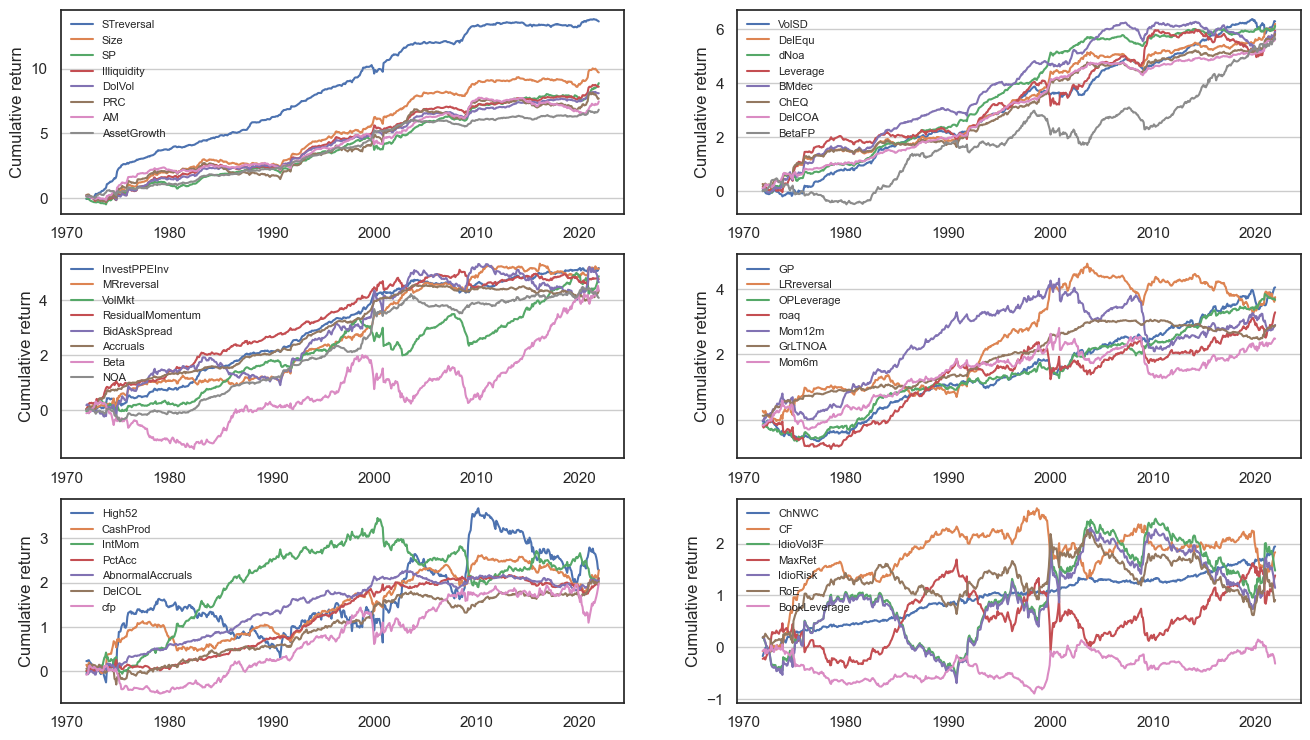
\includegraphics[width=.8\textwidth]{images/univariate_ls_cum_ret_capm.png}
  \label{fig: capm univariate ls cumulative return}
  \caption*{\footnotesize{This graphic showcases firm characteristics sorted univariate long-short portfolios' cumulative return acrossing the whole time period, the return refering to the abnormal return derived from CAPM factor model.}}
\end{figure}

\begin{figure}[H]
  \centering
  \caption{\textbf{CAPM Abnormal Return: Univariate Long-short Portfolios Performance in Different Macroeconomic Conditions}}
  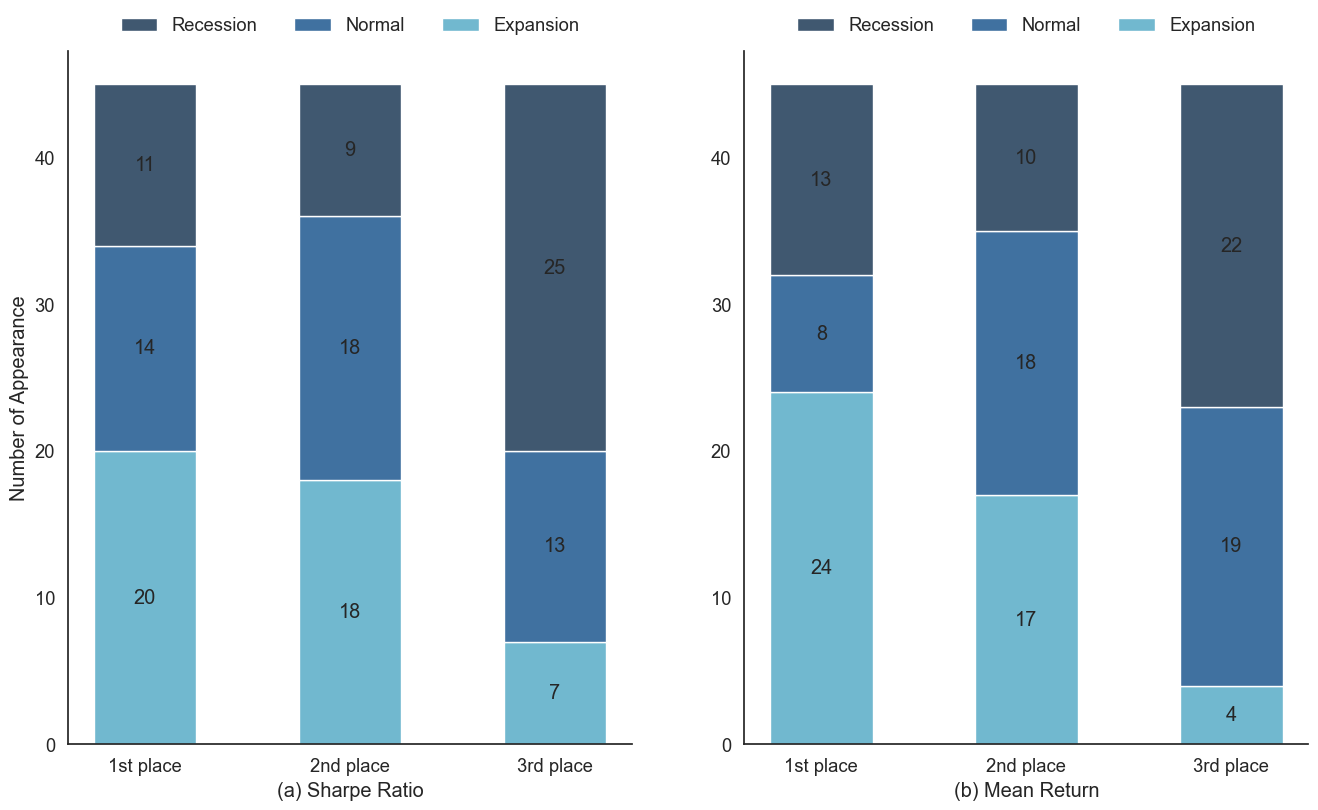
\includegraphics[width=.8\textwidth]{images/univariant_ls_capm_comparing.png}
  \label{fig: capm univariate ls comparing}
  \caption*{\footnotesize{This graphic showcases firm characteristics sorted long-short univariate portfolios' performance across different macroeconomic conditions. We compare univariate long-short portfolios' sharpe ratio and mean return in recession, normal, and expansion periods, which is the horizontal comparision among the last 6 columns in table \ref{table: capm univariate ls portfolio}.}}
\end{figure}

\begin{table}[H]
  \centering
  \footnotesize
  \caption{\textbf{CAPM Abnormal Return: Univariate Long-short Portfolios' Returns}}
  \label{table: capm univariate ls portfolio}
  \begin{tabular}{lcc|cc|cc|cc}
  \hline
      ~ & \multicolumn{2}{c}{Full Sample} & \multicolumn{2}{c}{Recession} & \multicolumn{2}{c}{Normal} & \multicolumn{2}{c}{Expansion} \\
      ~ & SR & Mean & SR & Mean & SR & Mean & SR & Mean \\ \hline
      STreversal & 0.023 & 0.364 & 0.037 & 0.485 & 0.012 & 0.219 & 0.018 & 0.367 \\ 
      Size & 0.010 & 0.302 & 0.009 & 0.258 & 0.008 & 0.272 & 0.013 & 0.372 \\ 
      Illiquidity & 0.009 & 0.289 & 0.008 & 0.224 & 0.007 & 0.279 & 0.013 & 0.366 \\ 
      DolVol & 0.010 & 0.270 & 0.005 & 0.121 & 0.014 & 0.465 & 0.013 & 0.292 \\ 
      High52 & 0.007 & 0.268 & 0.006 & 0.225 & 0.005 & 0.188 & 0.011 & 0.374 \\ 
      PRC & 0.011 & 0.257 & 0.009 & 0.200 & 0.013 & 0.305 & 0.012 & 0.276 \\ 
      SP & 0.009 & 0.253 & 0.007 & 0.185 & 0.008 & 0.303 & 0.010 & 0.304 \\ 
      BidAskSpread & 0.013 & 0.252 & 0.011 & 0.176 & 0.014 & 0.320 & 0.016 & 0.293 \\ 
      NOA & 0.015 & 0.239 & 0.014 & 0.193 & 0.014 & 0.238 & 0.016 & 0.323 \\ 
      VolSD & 0.010 & 0.233 & 0.011 & 0.223 & 0.009 & 0.241 & 0.011 & 0.240 \\ 
      dNoa & 0.010 & 0.228 & 0.011 & 0.231 & 0.007 & 0.202 & 0.011 & 0.248 \\ 
      InvestPPEInv & 0.014 & 0.225 & 0.012 & 0.178 & 0.015 & 0.293 & 0.015 & 0.228 \\ 
      DelCOA & 0.016 & 0.223 & 0.018 & 0.227 & 0.014 & 0.243 & 0.016 & 0.210 \\ 
      AssetGrowth & 0.010 & 0.209 & 0.002 & 0.032 & 0.012 & 0.285 & 0.016 & 0.366 \\ 
      AM & 0.008 & 0.194 & 0.005 & 0.098 & 0.006 & 0.199 & 0.013 & 0.314 \\ 
      OPLeverage & 0.005 & 0.187 & 0.003 & 0.121 & 0.003 & 0.150 & 0.008 & 0.273 \\ 
      Accruals & 0.012 & 0.185 & 0.014 & 0.167 & 0.008 & 0.130 & 0.015 & 0.275 \\ 
      GP & 0.009 & 0.177 & 0.011 & 0.203 & 0.005 & 0.137 & 0.009 & 0.180 \\ 
      BookLeverage & 0.007 & 0.166 & 0.011 & 0.250 & 0.004 & 0.091 & 0.006 & 0.147 \\ 
      DelEqu & 0.009 & 0.165 & 0.000 & -0.006 & 0.014 & 0.278 & 0.015 & 0.298 \\ 
      ChEQ & 0.007 & 0.165 & 0.003 & 0.067 & 0.011 & 0.262 & 0.007 & 0.183 \\ 
      Leverage & 0.010 & 0.163 & 0.010 & 0.134 & 0.006 & 0.100 & 0.014 & 0.271 \\ 
      ChNWC & 0.006 & 0.162 & 0.008 & 0.197 & 0.007 & 0.203 & 0.003 & 0.089 \\ 
      roaq & 0.003 & 0.152 & 0.006 & 0.261 & 0.000 & 0.024 & 0.003 & 0.140 \\ 
      MRreversal & 0.013 & 0.148 & 0.021 & 0.209 & 0.008 & 0.114 & 0.009 & 0.105 \\ 
      AbnormalAccruals & 0.003 & 0.146 & 0.005 & 0.189 & 0.000 & -0.009 & 0.005 & 0.218 \\ 
      GrLTNOA & 0.003 & 0.144 & 0.002 & 0.083 & 0.003 & 0.140 & 0.005 & 0.224 \\ 
      IdioVol3F & 0.008 & 0.133 & -0.005 & -0.070 & 0.014 & 0.315 & 0.016 & 0.275 \\ 
      BetaFP & 0.003 & 0.116 & 0.002 & 0.051 & 0.005 & 0.202 & 0.004 & 0.124 \\ 
      IdioRisk & 0.006 & 0.106 & 0.009 & 0.137 & 0.005 & 0.089 & 0.005 & 0.086 \\ 
      ResidualMomentum & 0.008 & 0.098 & 0.011 & 0.126 & 0.003 & 0.050 & 0.008 & 0.103 \\ 
      MaxRet & 0.004 & 0.097 & 0.003 & 0.060 & 0.001 & 0.042 & 0.007 & 0.209 \\ 
      CashProd & 0.005 & 0.090 & 0.000 & -0.006 & 0.011 & 0.216 & 0.006 & 0.103 \\ 
      DelCOL & 0.007 & 0.089 & 0.001 & 0.017 & 0.010 & 0.133 & 0.010 & 0.137 \\ 
      BMdec & 0.004 & 0.074 & -0.002 & -0.033 & 0.006 & 0.144 & 0.007 & 0.155 \\ 
      Beta & 0.005 & 0.071 & -0.004 & -0.051 & 0.011 & 0.196 & 0.009 & 0.166 \\ 
      PctAcc & 0.003 & 0.068 & -0.002 & -0.036 & 0.006 & 0.123 & 0.006 & 0.135 \\ 
      RoE & 0.004 & 0.064 & -0.004 & -0.043 & 0.010 & 0.202 & 0.007 & 0.132 \\ 
      cfp & 0.003 & 0.057 & -0.001 & -0.013 & 0.003 & 0.061 & 0.007 & 0.127 \\ 
      LRreversal & 0.004 & 0.046 & 0.021 & 0.193 & -0.008 & -0.123 & -0.003 & -0.041 \\ 
      CF & 0.002 & 0.034 & 0.001 & 0.010 & 0.002 & 0.032 & 0.004 & 0.058 \\ 
      Mom6m & 0.002 & 0.031 & 0.006 & 0.075 & 0.000 & 0.006 & 0.000 & 0.004 \\ 
      VolMkt & 0.002 & 0.025 & 0.008 & 0.118 & -0.004 & -0.071 & 0.000 & -0.002 \\ 
      Mom12m & 0.002 & 0.024 & 0.006 & 0.071 & 0.000 & -0.001 & 0.000 & -0.005 \\ 
      IntMom & -0.001 & -0.015 & 0.000 & 0.011 & 0.002 & 0.053 & -0.003 & -0.105 \\ \hline
  \end{tabular}
  \begin{tablenotes}
    \footnotesize
    \item This table presents firm characteristics sorted univariate long-short portfolios' sharpe ratios and mean returns. The dataset has futher splitted into three different subsamples based on macroeconomic condition indicator -- CFNAI index, named by recession, normal, and expansion period. The return in this table refering to the abnormal stock return derived from CAPM model.
  \end{tablenotes}
\end{table}

\begin{figure}[H]
  \centering
  \caption{\textbf{FF3 Abnormal Return: Univariate Long-short Portfolios' Cumulative Return}}
  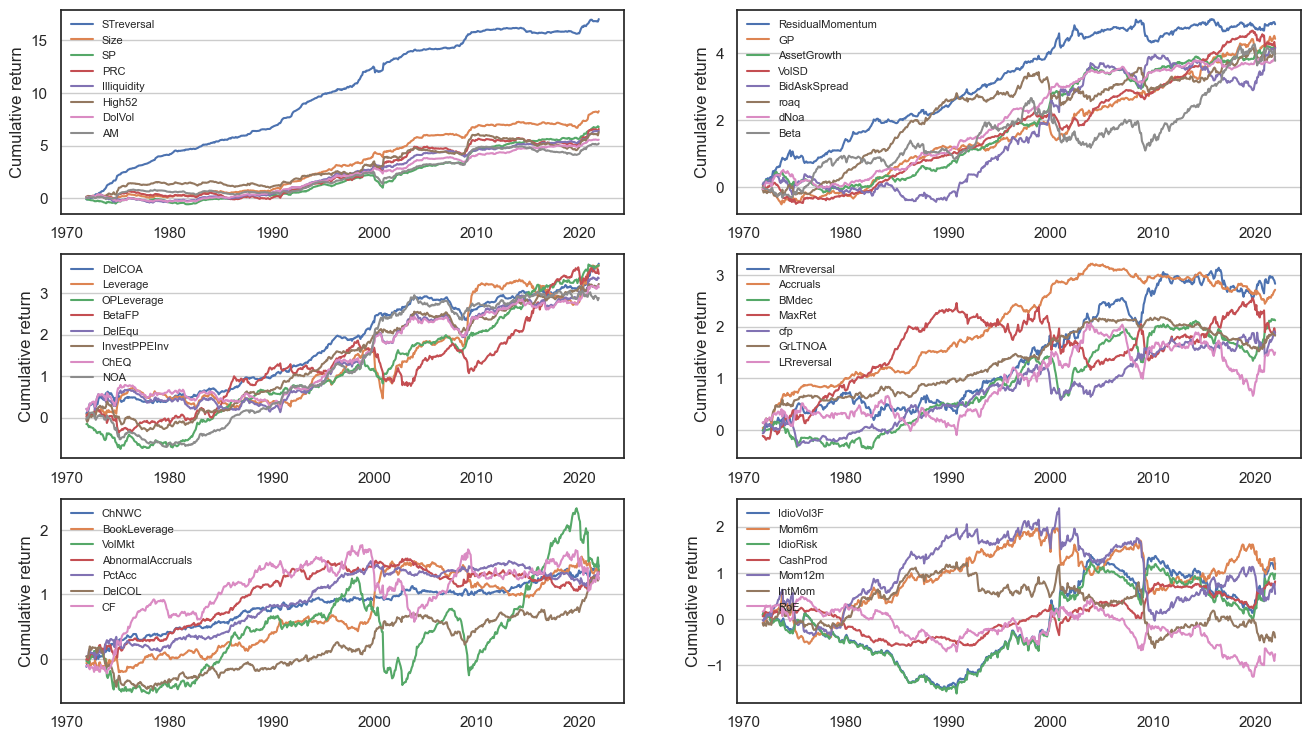
\includegraphics[width=.8\textwidth]{images/univariate_ls_cum_ret_ff3.png}
  \label{fig: ff3 univariate ls cumulative return}
  \caption*{\footnotesize{This graphic showcases firm characteristics sorted univariate long-short portfolios' cumulative return acrossing the whole time period, the return refering to the abnormal return derived from FF3 factor model.}}
\end{figure}

\begin{figure}[H]
  \centering
  \caption{\textbf{FF3 Abnormal Return: Univariate Long-short Portfolios Performance in Different Macroeconomic Conditions}}
  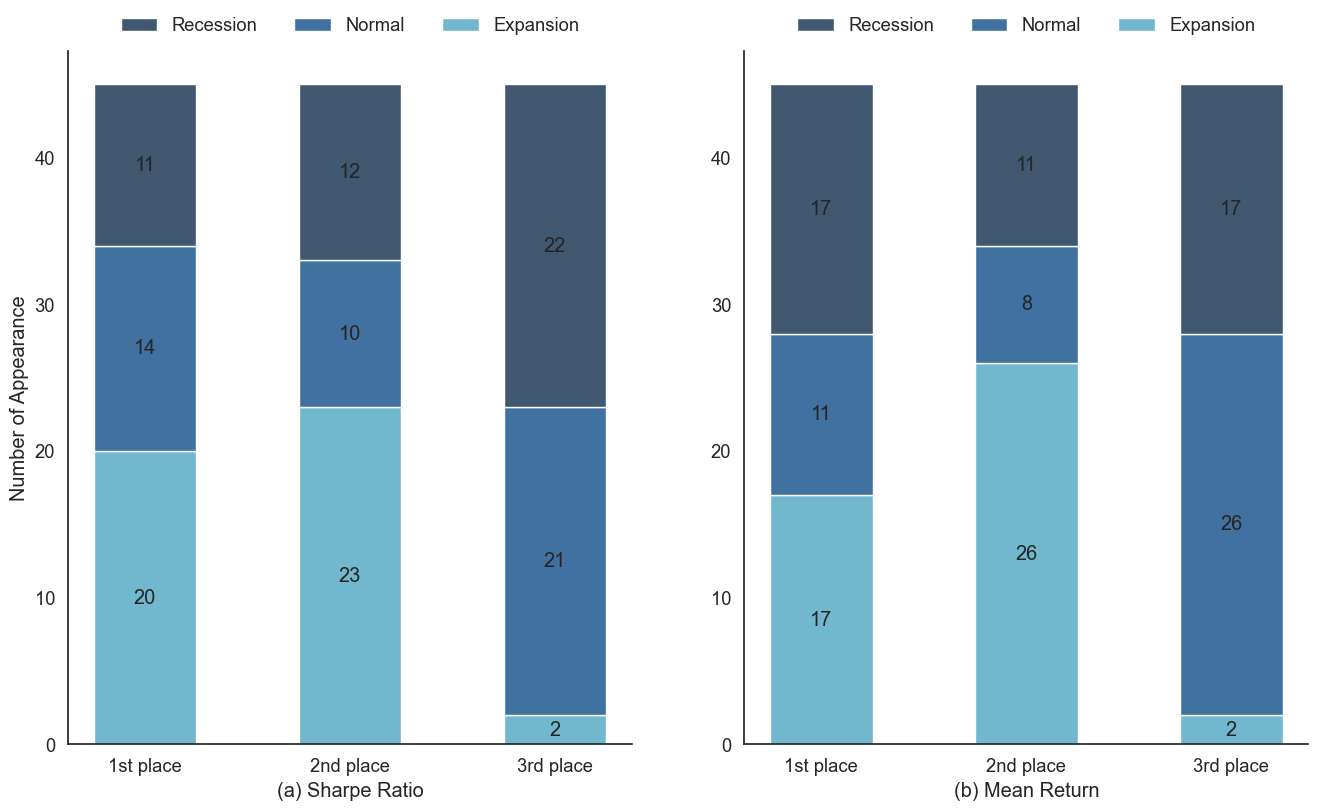
\includegraphics[width=.8\textwidth]{images/univariant_ls_ff3_comparing.png}
  \label{fig: ff3 univariate ls comparing}
  \caption*{\footnotesize{This graphic showcases firm characteristics sorted long-short univariate portfolios' performance across different macroeconomic conditions. We compare univariate long-short portfolios' sharpe ratio and mean return in recession, normal, and expansion periods, which is the horizontal comparision among the last 6 columns in table \ref{table: ff3 univariate ls portfolio}.}}
\end{figure}

\begin{table}[H]
  \centering
  \footnotesize
  \caption{\textbf{FF3 Abnormal Return: Univariate Long-short Portfolios' Returns}}
  \label{table: ff3 univariate ls portfolio}
  \begin{tabular}{lcc|cc|cc|cc}
  \hline
      ~ & \multicolumn{2}{c}{Full Sample} & \multicolumn{2}{c}{Recession} & \multicolumn{2}{c}{Normal} & \multicolumn{2}{c}{Expansion} \\
      ~ & SR & Mean & SR & Mean & SR & Mean & SR & Mean \\ \hline
      STreversal & 0.028 & 0.447 & 0.036 & 0.468 & 0.018 & 0.333 & 0.029 & 0.559 \\ 
      Size & 0.014 & 0.238 & 0.014 & 0.216 & 0.012 & 0.241 & 0.015 & 0.265 \\ 
      SP & 0.011 & 0.221 & 0.012 & 0.184 & 0.010 & 0.236 & 0.011 & 0.293 \\ 
      Illiquidity & 0.011 & 0.218 & 0.008 & 0.143 & 0.011 & 0.273 & 0.013 & 0.267 \\ 
      DolVol & 0.009 & 0.216 & 0.006 & 0.128 & 0.010 & 0.264 & 0.012 & 0.283 \\ 
      dNoa & 0.006 & 0.210 & 0.007 & 0.217 & 0.003 & 0.121 & 0.009 & 0.276 \\ 
      DelCOA & 0.006 & 0.202 & 0.006 & 0.189 & 0.003 & 0.120 & 0.009 & 0.274 \\ 
      VolSD & 0.007 & 0.191 & 0.001 & 0.037 & 0.011 & 0.354 & 0.009 & 0.235 \\ 
      GP & 0.007 & 0.184 & 0.005 & 0.118 & 0.011 & 0.258 & 0.007 & 0.183 \\ 
      AssetGrowth & 0.007 & 0.181 & 0.007 & 0.172 & 0.007 & 0.184 & 0.007 & 0.188 \\ 
      ResidualMomentum & 0.008 & 0.178 & 0.004 & 0.080 & 0.007 & 0.201 & 0.012 & 0.293 \\ 
      InvestPPEInv & 0.005 & 0.174 & 0.006 & 0.160 & 0.005 & 0.172 & 0.006 & 0.193 \\ 
      Accruals & 0.005 & 0.170 & 0.005 & 0.185 & 0.001 & 0.036 & 0.007 & 0.258 \\ 
      OPLeverage & 0.006 & 0.168 & 0.008 & 0.206 & 0.007 & 0.209 & 0.003 & 0.094 \\ 
      AM & 0.009 & 0.154 & 0.011 & 0.150 & 0.004 & 0.084 & 0.010 & 0.248 \\ 
      PRC & 0.011 & 0.149 & 0.018 & 0.207 & 0.006 & 0.087 & 0.009 & 0.132 \\ 
      DelEqu & 0.006 & 0.141 & 0.008 & 0.190 & 0.003 & 0.093 & 0.005 & 0.129 \\ 
      ChEQ & 0.005 & 0.136 & 0.009 & 0.198 & 0.001 & 0.044 & 0.005 & 0.137 \\ 
      NOA & 0.005 & 0.136 & 0.009 & 0.228 & 0.002 & 0.051 & 0.003 & 0.095 \\ 
      High52 & 0.010 & 0.133 & 0.022 & 0.222 & 0.000 & -0.006 & 0.008 & 0.136 \\ 
      roaq & 0.007 & 0.129 & 0.000 & 0.006 & 0.012 & 0.266 & 0.008 & 0.164 \\ 
      BetaFP & 0.006 & 0.124 & -0.003 & -0.060 & 0.012 & 0.314 & 0.009 & 0.217 \\ 
      Leverage & 0.006 & 0.121 & 0.007 & 0.104 & 0.002 & 0.040 & 0.009 & 0.247 \\ 
      GrLTNOA & 0.003 & 0.118 & 0.003 & 0.112 & 0.001 & 0.033 & 0.005 & 0.182 \\ 
      ChNWC & 0.002 & 0.113 & 0.005 & 0.216 & 0.000 & -0.021 & 0.003 & 0.114 \\ 
      BidAskSpread & 0.007 & 0.106 & 0.010 & 0.129 & 0.003 & 0.046 & 0.008 & 0.129 \\ 
      MRreversal & 0.005 & 0.097 & 0.008 & 0.139 & 0.001 & 0.025 & 0.005 & 0.106 \\ 
      BMdec & 0.004 & 0.096 & -0.003 & -0.079 & 0.005 & 0.127 & 0.009 & 0.300 \\ 
      AbnormalAccruals & 0.002 & 0.094 & 0.004 & 0.135 & -0.001 & -0.066 & 0.004 & 0.168 \\ 
      PctAcc & 0.002 & 0.093 & 0.001 & 0.043 & 0.001 & 0.050 & 0.004 & 0.181 \\ 
      Beta & 0.006 & 0.091 & 0.000 & 0.004 & 0.014 & 0.212 & 0.005 & 0.085 \\ 
      BookLeverage & 0.002 & 0.081 & 0.003 & 0.082 & 0.005 & 0.200 & 0.000 & -0.011 \\ 
      DelCOL & 0.002 & 0.077 & 0.002 & 0.054 & 0.002 & 0.101 & 0.002 & 0.081 \\ 
      cfp & 0.003 & 0.074 & -0.001 & -0.015 & 0.004 & 0.110 & 0.006 & 0.147 \\ 
      MaxRet & 0.003 & 0.057 & 0.001 & 0.009 & 0.004 & 0.096 & 0.005 & 0.091 \\ 
      LRreversal & 0.002 & 0.046 & 0.008 & 0.130 & -0.003 & -0.059 & 0.002 & 0.046 \\ 
      CF & 0.002 & 0.044 & -0.003 & -0.051 & 0.004 & 0.095 & 0.005 & 0.110 \\ 
      VolMkt & 0.002 & 0.043 & -0.008 & -0.121 & 0.008 & 0.212 & 0.007 & 0.142 \\ 
      CashProd & 0.001 & 0.043 & 0.000 & 0.012 & 0.000 & -0.012 & 0.004 & 0.150 \\ 
      IdioVol3F & 0.002 & 0.032 & 0.006 & 0.081 & -0.001 & -0.025 & 0.001 & 0.015 \\ 
      Mom6m & 0.002 & 0.028 & -0.005 & -0.064 & 0.006 & 0.108 & 0.005 & 0.096 \\ 
      IdioRisk & 0.002 & 0.026 & 0.006 & 0.082 & -0.002 & -0.030 & 0.000 & 0.001 \\ 
      Mom12m & 0.001 & 0.012 & -0.008 & -0.083 & 0.007 & 0.124 & 0.004 & 0.068 \\ 
      IntMom & -0.001 & -0.012 & -0.005 & -0.074 & 0.003 & 0.074 & 0.000 & 0.001 \\ 
      RoE & -0.001 & -0.025 & 0.006 & 0.103 & -0.006 & -0.141 & -0.004 & -0.078 \\ \hline
  \end{tabular}
  \begin{tablenotes}
    \footnotesize
    \item This table presents firm characteristics sorted univariate long-short portfolios' sharpe ratios and mean returns. The dataset has futher splitted into three different subsamples based on macroeconomic condition indicator -- CFNAI index, named by recession, normal, and expansion period. The return in this table refering to the abnormal stock return derived from FF3 factors model.
  \end{tablenotes}
\end{table}

\begin{figure}[H]
  \centering
  \caption{\textbf{Excess Return: Univariate Long-short Portfolios' Cumulative Return}}
  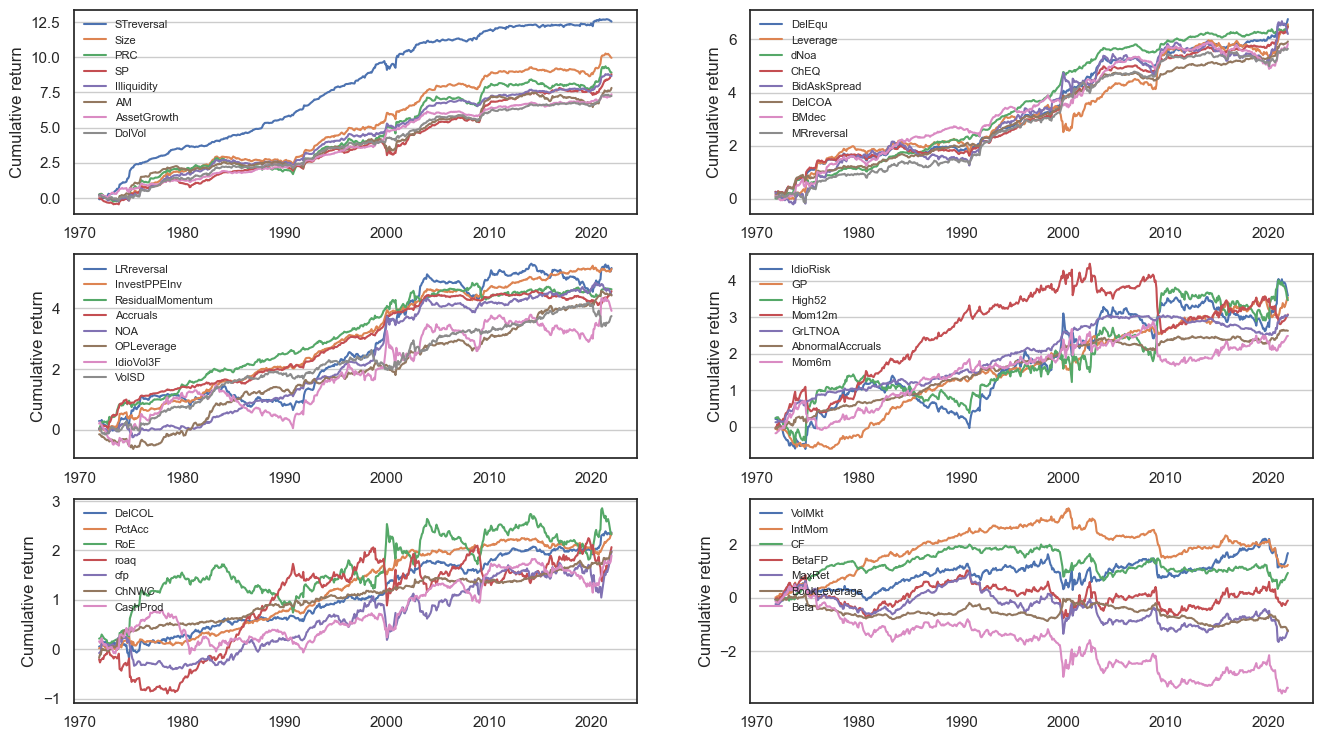
\includegraphics[width=.8\textwidth]{images/univariate_ls_cum_ret_excess.png}
  \label{fig: excess univariate ls cumulative return}
  \caption*{\footnotesize{This graphic showcases firm characteristics sorted univariate long-short portfolios' cumulative return acrossing the whole time period, the return refering to the stock excess return.}}
\end{figure}

\begin{figure}[H]
  \centering
  \caption{\textbf{Excess Return: Univariate Long-short Portfolios Performance in Different Macroeconomic Conditions}}
  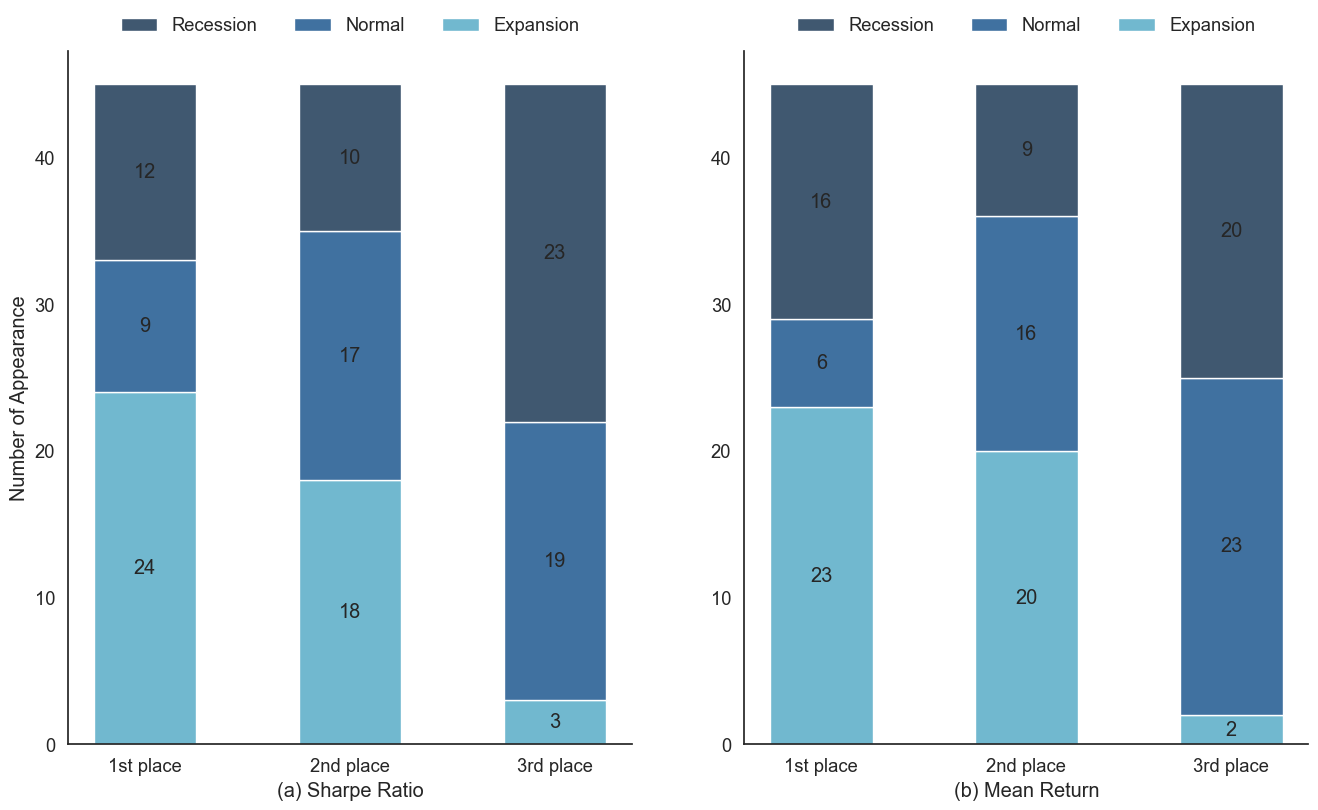
\includegraphics[width=.8\textwidth]{images/univariant_ls_excess_comparing.png}
  \label{fig: excess univariate ls comparing}
  \caption*{\footnotesize{This graphic showcases firm characteristics sorted long-short univariate portfolios' performance across different macroeconomic conditions. We compare univariate long-short portfolios' sharpe ratio and mean return in recession, normal, and expansion periods, which is the horizontal comparision among the last 6 columns in table \ref{table: excess univariate ls portfolio}.}}
\end{figure}

\begin{table}[H]
  \centering
  \footnotesize
  \caption{\textbf{Excess Return: Univariate Long-short Portfolios' Returns}}
  \label{table: excess univariate ls portfolio}
  \begin{tabular}{lcc|cc|cc|cc}
  \hline
      ~ & \multicolumn{2}{c}{Full Sample} & \multicolumn{2}{c}{Recession} & \multicolumn{2}{c}{Normal} & \multicolumn{2}{c}{Expansion} \\
      STreversal & 0.021 & 0.323 & 0.034 & 0.412 & 0.012 & 0.218 & 0.016 & 0.326 \\ 
      dNoa & 0.011 & 0.314 & 0.010 & 0.259 & 0.009 & 0.282 & 0.014 & 0.403 \\ 
      DelCOA & 0.010 & 0.296 & 0.009 & 0.246 & 0.007 & 0.256 & 0.014 & 0.377 \\ 
      AssetGrowth & 0.012 & 0.278 & 0.011 & 0.231 & 0.013 & 0.306 & 0.013 & 0.303 \\ 
      Accruals & 0.008 & 0.264 & 0.007 & 0.220 & 0.004 & 0.166 & 0.012 & 0.386 \\ 
      InvestPPEInv & 0.009 & 0.256 & 0.007 & 0.184 & 0.008 & 0.308 & 0.010 & 0.314 \\ 
      DelEqu & 0.011 & 0.253 & 0.012 & 0.253 & 0.009 & 0.243 & 0.012 & 0.262 \\ 
      ChEQ & 0.011 & 0.249 & 0.012 & 0.261 & 0.008 & 0.217 & 0.012 & 0.263 \\ 
      Size & 0.017 & 0.233 & 0.019 & 0.245 & 0.014 & 0.239 & 0.016 & 0.221 \\ 
      Illiquidity & 0.014 & 0.231 & 0.013 & 0.196 & 0.014 & 0.272 & 0.016 & 0.241 \\ 
      SP & 0.015 & 0.228 & 0.016 & 0.204 & 0.013 & 0.218 & 0.015 & 0.287 \\ 
      DolVol & 0.012 & 0.225 & 0.010 & 0.168 & 0.011 & 0.245 & 0.015 & 0.276 \\ 
      MRreversal & 0.009 & 0.193 & 0.014 & 0.244 & 0.004 & 0.087 & 0.010 & 0.220 \\ 
      OPLeverage & 0.007 & 0.193 & 0.009 & 0.220 & 0.008 & 0.235 & 0.005 & 0.128 \\ 
      BMdec & 0.010 & 0.192 & 0.002 & 0.042 & 0.012 & 0.270 & 0.015 & 0.318 \\ 
      GrLTNOA & 0.005 & 0.190 & 0.004 & 0.166 & 0.002 & 0.089 & 0.009 & 0.280 \\ 
      ResidualMomentum & 0.008 & 0.185 & 0.001 & 0.029 & 0.009 & 0.256 & 0.013 & 0.346 \\ 
      AM & 0.013 & 0.184 & 0.017 & 0.195 & 0.007 & 0.114 & 0.014 & 0.243 \\ 
      AbnormalAccruals & 0.004 & 0.178 & 0.005 & 0.200 & 0.001 & 0.065 & 0.006 & 0.237 \\ 
      NOA & 0.007 & 0.177 & 0.010 & 0.218 & 0.005 & 0.118 & 0.007 & 0.185 \\ 
      Leverage & 0.011 & 0.169 & 0.013 & 0.168 & 0.006 & 0.103 & 0.013 & 0.239 \\ 
      PRC & 0.015 & 0.169 & 0.024 & 0.230 & 0.008 & 0.124 & 0.011 & 0.135 \\ 
      PctAcc & 0.004 & 0.155 & 0.003 & 0.097 & 0.003 & 0.158 & 0.006 & 0.234 \\ 
      LRreversal & 0.009 & 0.149 & 0.013 & 0.194 & 0.006 & 0.119 & 0.008 & 0.125 \\ 
      ChNWC & 0.003 & 0.147 & 0.005 & 0.223 & 0.000 & 0.027 & 0.004 & 0.159 \\ 
      GP & 0.006 & 0.144 & 0.003 & 0.071 & 0.009 & 0.206 & 0.006 & 0.169 \\ 
      DelCOL & 0.004 & 0.135 & 0.003 & 0.085 & 0.005 & 0.197 & 0.004 & 0.145 \\ 
      BidAskSpread & 0.010 & 0.127 & 0.014 & 0.155 & 0.004 & 0.067 & 0.012 & 0.142 \\ 
      VolSD & 0.006 & 0.126 & 0.001 & 0.016 & 0.009 & 0.223 & 0.009 & 0.187 \\ 
      IdioVol3F & 0.007 & 0.076 & 0.012 & 0.124 & 0.003 & 0.045 & 0.004 & 0.047 \\ 
      CashProd & 0.003 & 0.074 & 0.003 & 0.054 & 0.001 & 0.028 & 0.005 & 0.139 \\ 
      IdioRisk & 0.006 & 0.071 & 0.012 & 0.122 & 0.003 & 0.039 & 0.003 & 0.039 \\ 
      Mom12m & 0.005 & 0.068 & -0.005 & -0.054 & 0.011 & 0.183 & 0.010 & 0.186 \\ 
      cfp & 0.003 & 0.065 & -0.001 & -0.026 & 0.005 & 0.114 & 0.006 & 0.134 \\ 
      RoE & 0.004 & 0.063 & 0.010 & 0.149 & -0.001 & -0.024 & 0.002 & 0.037 \\ 
      High52 & 0.006 & 0.062 & 0.024 & 0.193 & -0.006 & -0.089 & -0.002 & -0.026 \\ 
      Mom6m & 0.004 & 0.059 & -0.005 & -0.057 & 0.012 & 0.225 & 0.007 & 0.133 \\ 
      roaq & 0.003 & 0.055 & -0.003 & -0.040 & 0.010 & 0.175 & 0.004 & 0.072 \\ 
      IntMom & 0.002 & 0.039 & -0.004 & -0.066 & 0.004 & 0.088 & 0.006 & 0.140 \\ 
      VolMkt & 0.003 & 0.036 & -0.010 & -0.102 & 0.008 & 0.139 & 0.011 & 0.162 \\ 
      CF & 0.002 & 0.028 & -0.002 & -0.033 & 0.002 & 0.041 & 0.005 & 0.085 \\ 
      BetaFP & 0.000 & -0.002 & -0.011 & -0.110 & 0.004 & 0.066 & 0.007 & 0.104 \\ 
      MaxRet & -0.002 & -0.027 & -0.006 & -0.073 & -0.001 & -0.008 & 0.000 & 0.005 \\ 
      BookLeverage & -0.002 & -0.058 & -0.003 & -0.062 & 0.000 & -0.003 & -0.003 & -0.102 \\ 
      Beta & -0.006 & -0.066 & -0.013 & -0.126 & -0.003 & -0.037 & -0.001 & -0.013 \\ \hline
  \end{tabular}
  \begin{tablenotes}
    \footnotesize
    \item This table presents firm characteristics sorted univariate long-short portfolios' sharpe ratios and mean returns. The dataset has futher splitted into three different subsamples based on macroeconomic condition indicator -- CFNAI index, named by recession, normal, and expansion period. The return in this table refering to the stock excess return.
  \end{tablenotes}
\end{table}

%%%%%%%%%%%%%%%%%%%%%%%%%%%%%%%%%%%%%%%%%%%%%%%%%%%%%%%%%%%%%%%%%%%%%%%%%%%%%%%%%%%%%%%%
\subsection*{B2. Robust Result for Predictions Based Portfolios}\label{sec:appendixb2}

\begin{figure}[H]
  \centering
  \caption{\textbf{Cumulative Return of Portfolios Based on Prediction with Firm Features and CFNAI}}
  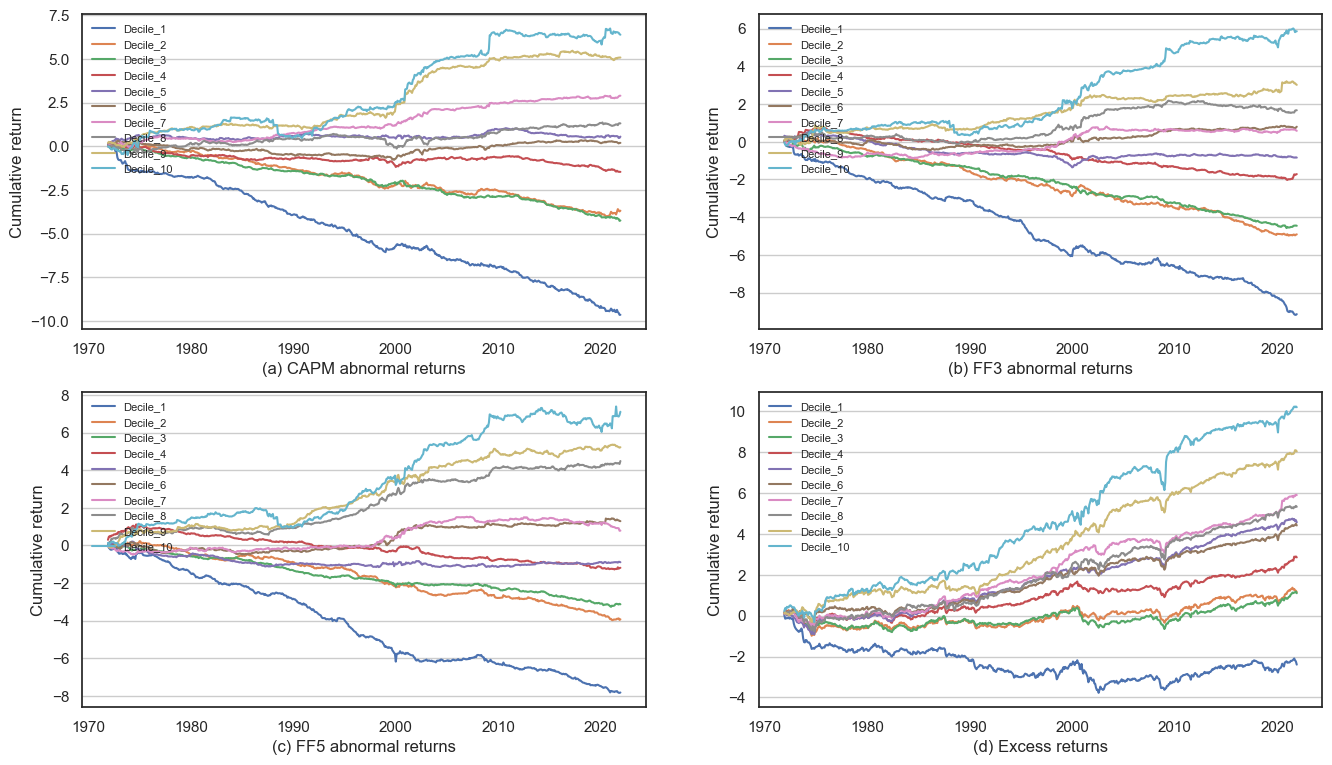
\includegraphics[width=.8\textwidth]{images/vw_portfolios_cumulative_return_cfnai.png}
  \label{fig: portfolios cum return firm features and cfnai}
  \caption*{\footnotesize{This graphic shows the cumulative return of value weighted portfolios based on predictions with firm characteristic feature variables and CFNAI data.}}
\end{figure}

\begin{figure}[H]
  \centering
  \caption{\textbf{Cumulative Return of Portfolios Based on Prediction with Firm Features and Sentiment}}
  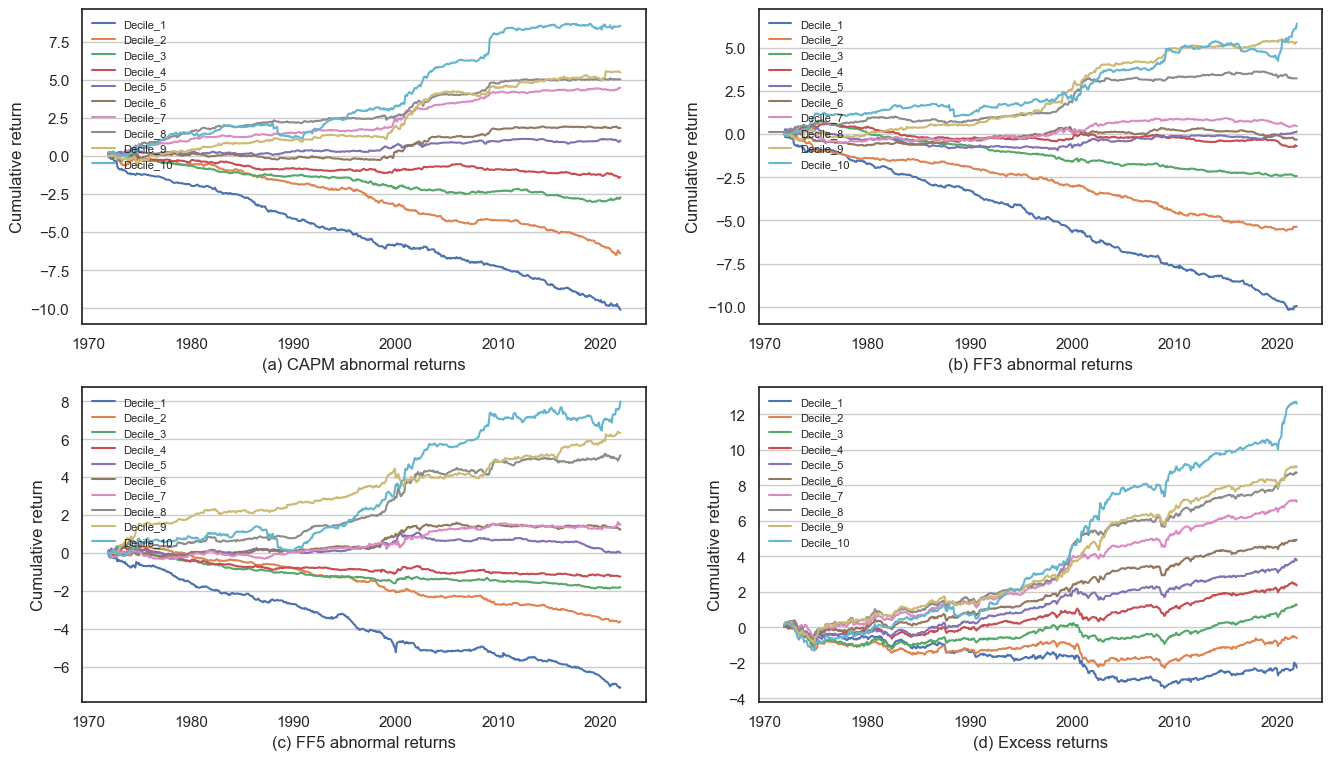
\includegraphics[width=.8\textwidth]{images/vw_portfolios_cumulative_return_sent.png}
  \label{fig: portfolios cum return firm features and sent}
  \caption*{\footnotesize{This graphic shows the cumulative return of value weighted portfolios based on predictions with firm characteristic feature variables and investors sentiment data.}}
\end{figure}

%%%%%%%%%%%%%%%%%%%%%%%%%%%%%%%%%%%%%%%%%%%%%%%%%%%%%%%%%%%%%%%%%%%%%%%%%%%%%%%%%%%%%%%%
\subsection*{B3. Robust Result for Feature Importance}
\label{sec:appendixb3}

\begin{figure}[H]
  \centering
  \caption{\textbf{Shap Feature Importance for CAPM Abnormal Return}}
  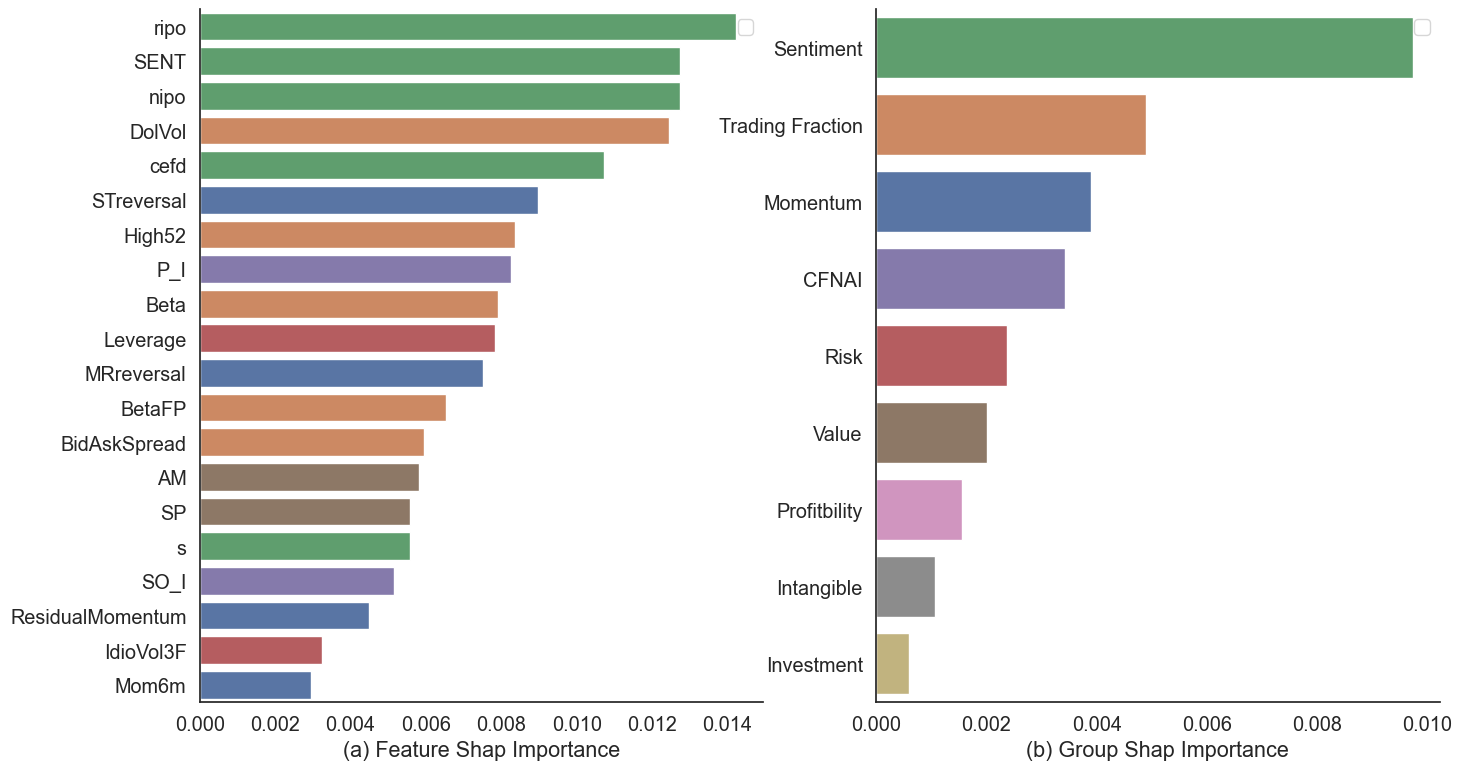
\includegraphics[width=.8\textwidth]{images/shap_feature_importance_capm.png}
  \label{fig: feature importance capm}
  \caption*{\footnotesize{This figure shows the importance ranking for predictor variables and variable groups in predicitng stock abnormal returns derived CAPM factor model. The ranking is the average of the feature variables' Shap force. The variable importance measures are evaluated on the testing dataset. Group shap importance is the feature importance's sum value within each group.}}
\end{figure}

\begin{figure}[H]
  \centering
  \caption{\textbf{Shap Feature Importance for FF3 Abnormal Return}}
  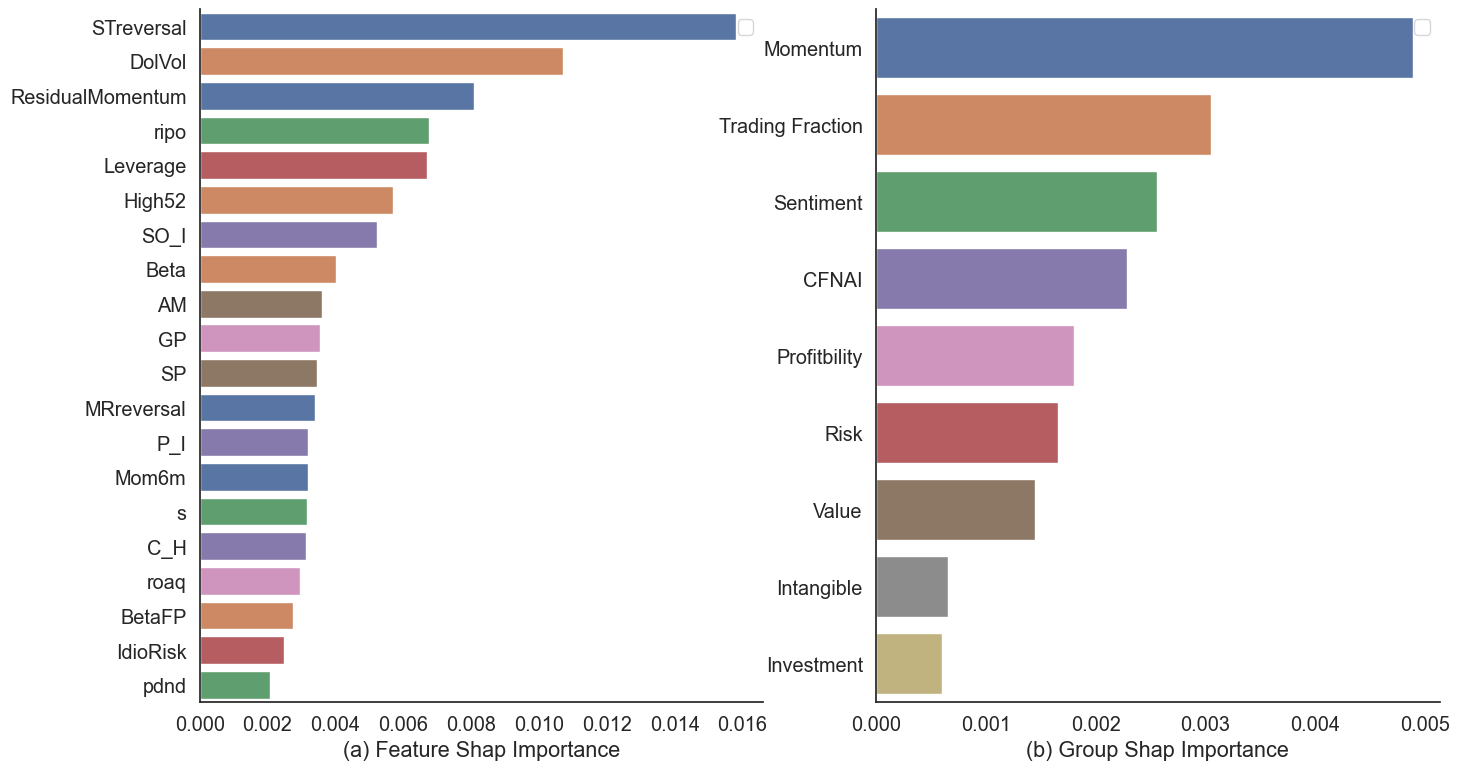
\includegraphics[width=.8\textwidth]{images/shap_feature_importance_ff3.png}
  \label{fig: feature importance ff3}
  \caption*{\footnotesize{This figure shows the importance ranking for predictor variables and variable groups in predicitng stock abnormal returns derived FF3 factors model. The ranking is the average of the feature variables' Shap force. The variable importance measures are evaluated on the testing dataset. Group shap importance is the feature importance's sum value within each group.}}
\end{figure}

%%%%%%%%%%%%%%%%%%%%%%%%%%%%%%%%%%%%%%%%%%%%%%%%%%%%%%%%%%%%%%%%%%%%%%%%%%%%%%%%%%%%%%%%
\subsection*{B4. Robust Result for Interaction Effects}
\label{sec:appendixb4}

\begin{figure}[H]
  \centering
  \caption{\textbf{Interaction Effects Between Firm Features and CFNAI, FF3}}
  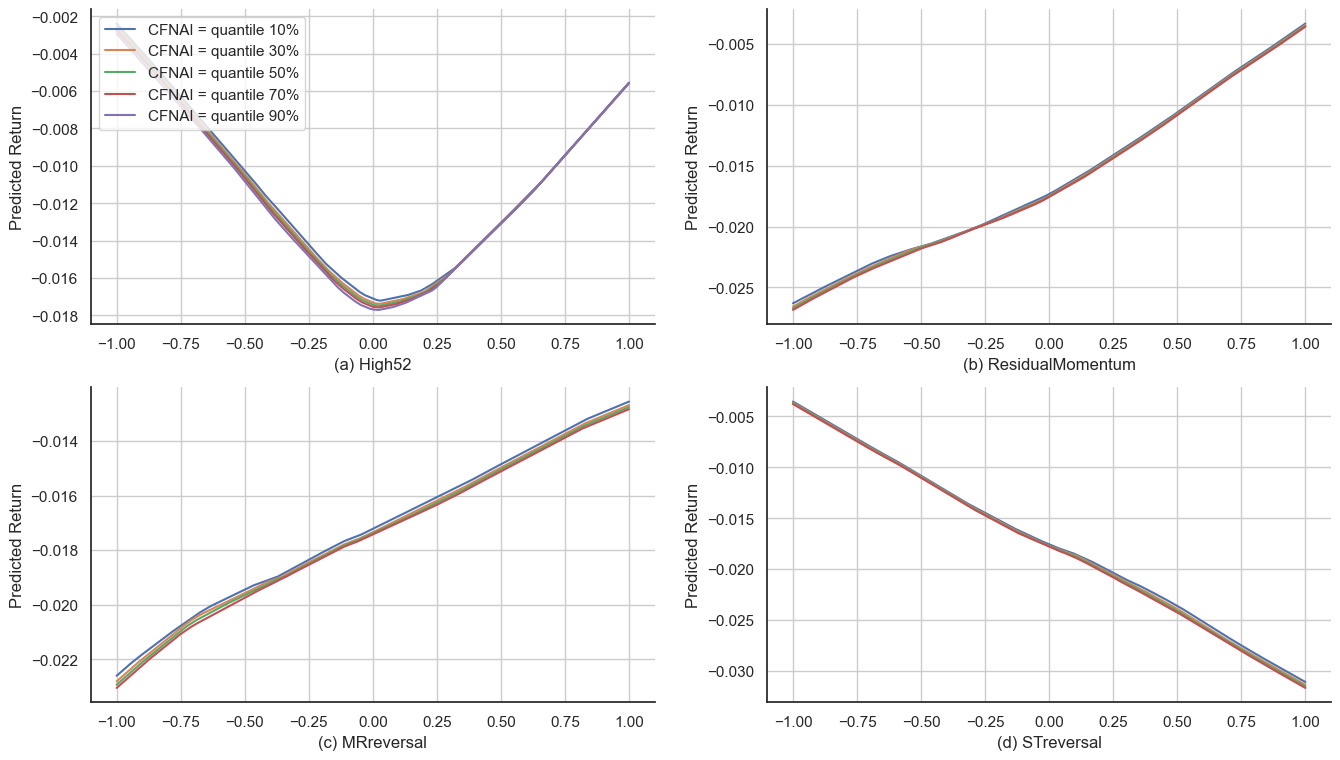
\includegraphics[width=.8\textwidth]{images/interactive_effect_ff3.png}
  \label{fig: interaction effect_ff3}
  \caption*{\footnotesize{This graphic shows the predicted stock abnormal return derived from FF3 factors model as a function of one stock characteristic feature variable, High52 (52 weeks trading high), ResidualMomentum (Momentum based on FF3 residuals  ), MRreversal (Medium‐run reversal), STreversal (Short term reversal) accordingly. The 'one' variable has a range between(-1, 1), macroeconomic variable CFNAI is seperated at 10\%, 30\%, 50\%, 70\%, and 90\% level. All other variables are fixed with the median value in the testing dataset.}}
\end{figure}

\begin{figure}[H]
  \centering
  \caption{\textbf{Interaction Effects Between Firm Features and CFNAI, CAPM}}
  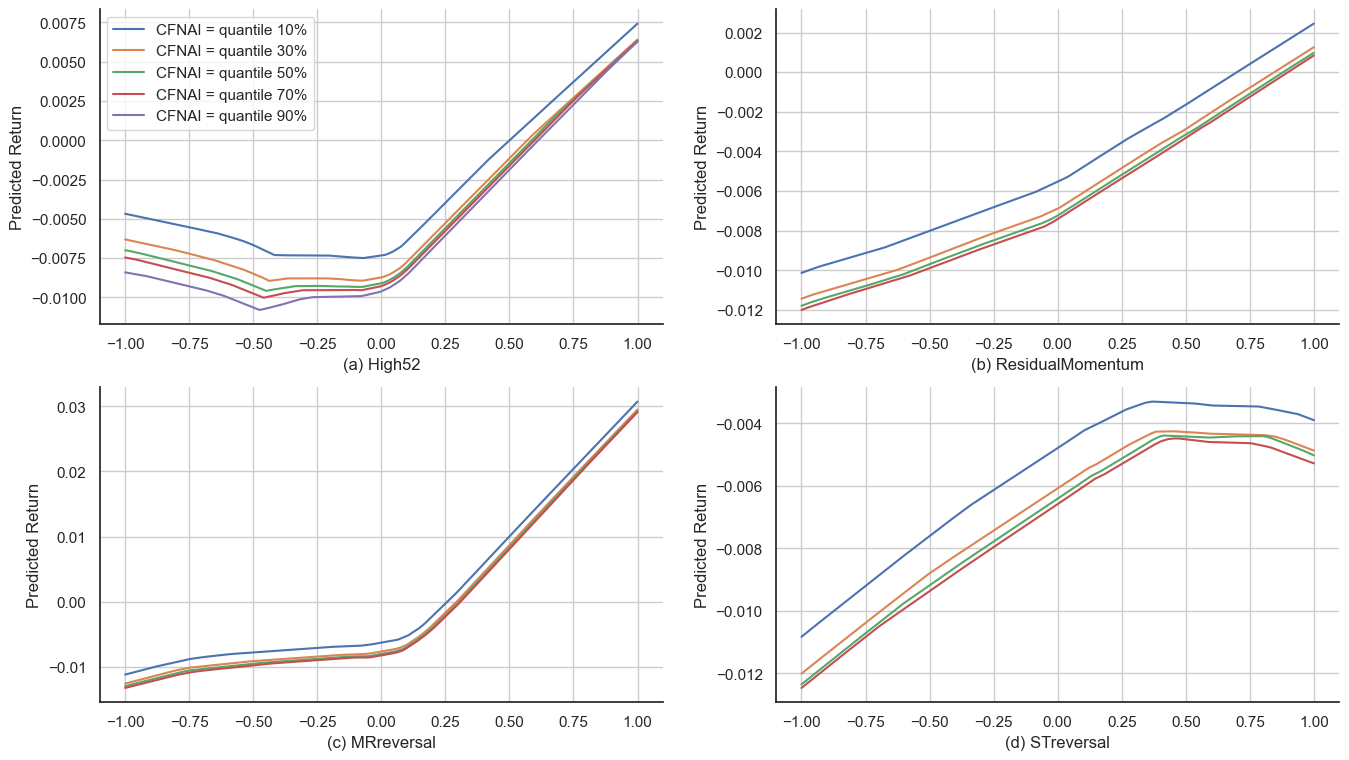
\includegraphics[width=.8\textwidth]{images/interactive_effect_capm.png}
  \label{fig: interaction effect_capm}
  \caption*{\footnotesize{This graphic shows the predicted stock abnormal return derived from CAPM model as a function of one stock characteristic feature variable, High52 (52 weeks trading high), ResidualMomentum (Momentum based on FF3 residuals  ), MRreversal (Medium‐run reversal), STreversal (Short term reversal) accordingly. The 'one' variable has a range between(-1, 1), macroeconomic variable CFNAI is seperated at 10\%, 30\%, 50\%, 70\%, and 90\% level. All other variables are fixed with the median value in the testing dataset.}}
\end{figure}

%%%%%%%%%%%%%%%%%%%%%%%%%%%%%%%%%%%%%%%%%%%%%%%%%%%%%%%%%%%%%%%%%%%%%%%%%%%%%%%%%%%%%%%%
\subsection*{B4. Robust Result for Market Timing}
\label{sec:appendixb5}

\begin{table}[H]
  \centering
  \caption{\textbf{Prediction Based Portfolios' Return in Defferent Macroeconomic Conditions}}
  \begin{tabular}{l|cc|cc|cc}
  \hline
      \multicolumn{7}{c}{(a) Portfolios' CAMP Abnormal Return (Mean)}\\\hline
      ~ & \multicolumn{2}{c}{Recession} & \multicolumn{2}{c}{Normal} & \multicolumn{2}{c}{Expansion} \\ \cline{2-7}
      Portfolios & Mean & Sharpe Ratio & Mean & Sharpe Ratio & Mean & Sharpe Ratio \\ \hline
      Decile\_1 & -1.503 & -0.338 & -1.263 & -0.275 & -1.035 & -0.195 \\ 
      Decile\_2 & -0.443 & -0.153 & -0.477 & -0.163 & -0.717 & -0.223 \\ 
      Decile\_3 & -0.333 & -0.123 & -0.252 & -0.113 & -0.463 & -0.145 \\ 
      Decile\_4 & -0.231 & -0.079 & -0.236 & -0.123 & -0.294 & -0.097 \\ 
      Decile\_5 & -0.111 & -0.035 & -0.050 & -0.024 & -0.273 & -0.087 \\ 
      Decile\_6 & 0.341 & 0.090 & 0.026 & 0.010 & -0.146 & -0.043 \\ 
      Decile\_7 & 0.443 & 0.121 & 0.156 & 0.057 & -0.220 & -0.065 \\ 
      Decile\_8 & 0.504 & 0.102 & 0.272 & 0.092 & 0.173 & 0.042 \\ 
      Decile\_9 & 1.331 & 0.238 & 0.616 & 0.176 & 0.438 & 0.091 \\ 
      Decile\_10 & 3.123 & 0.326 & 1.584 & 0.313 & 1.682 & 0.266 \\  \hline

      \multicolumn{7}{c}{(b) Portfolios' FF3 Abnormal Return (Mean)}\\\hline
      ~ & \multicolumn{2}{c}{Recession} & \multicolumn{2}{c}{Normal} & \multicolumn{2}{c}{Expansion} \\ \cline{2-7}
      Portfolios & Mean & Sharpe Ratio & Mean & Sharpe Ratio & Mean & Sharpe Ratio \\ \hline
      Decile\_1 & -1.778 & -0.397 & -1.642 & -0.533 & -1.485 & -0.382 \\ 
      Decile\_2 & -0.708 & -0.275 & -0.655 & -0.409 & -1.003 & -0.442 \\ 
      Decile\_3 & -0.656 & -0.301 & -0.371 & -0.261 & -0.564 & -0.237 \\ 
      Decile\_4 & -0.457 & -0.220 & -0.384 & -0.233 & -0.302 & -0.131 \\ 
      Decile\_5 & -0.334 & -0.143 & -0.200 & -0.123 & -0.200 & -0.084 \\ 
      Decile\_6 & 0.125 & 0.050 & -0.065 & -0.036 & -0.055 & -0.023 \\ 
      Decile\_7 & 0.168 & 0.061 & 0.120 & 0.061 & 0.003 & 0.002 \\ 
      Decile\_8 & 0.142 & 0.041 & 0.218 & 0.110 & 0.404 & 0.147 \\ 
      Decile\_9 & 1.021 & 0.243 & 0.616 & 0.205 & 0.784 & 0.244 \\ 
      Decile\_10 & 2.738 & 0.361 & 1.661 & 0.338 & 2.019 & 0.408 \\  \hline
  \end{tabular}
  \label{table: portfolio ret in tertiles rest}
  \begin{tablenotes}
    \footnotesize
    \item This table presents the actual mean portfolios' return and sharpe ratio in different macroeconomic conbinations. Portfolios are sorted based on the predicted abnormal and excess stock return made by neural network model. Macroeconomic conbinations defined as recession period, normal period, and expansion period based on the CFNAI index.
  \end{tablenotes}
\end{table}